\section{Results}
\label{sec:results}

This chapter reports the empirical findings used to answer the research questions.
The emphasis here is descriptive and comparative.
Broader interpretation is deferred to \Cref{sec:discussion}.
All numbers are derived from the frozen results pack and the report-ready imports under \texttt{report/figures/final\_pack/} and \texttt{report/tables/final\_pack/}.

\subsection{Baseline model behaviour and evaluation set}
All experiments use the CIFAR-10 test set restricted to indices 0--9{,}999.
Under the fixed pretrained classifier, 9{,}213 of these 10{,}000 images are classified correctly and are therefore eligible for attack.
This corresponds to a clean accuracy of 92.13\% on the fixed evaluation range.
The eligible subset is reused consistently across all attack variants.

This detail matters because the headline attack success rates in the chapter are not percentages over the entire 10k image set.
They are percentages over the 9{,}213 images for which the classifier is initially correct.
Attack success therefore always means overturning a correct clean prediction rather than merely changing the output on an already misclassified image.

\subsection{Artefact coverage and consistency checks}
The frozen artefacts also provide a useful internal consistency check between attack outputs and explanation outputs.
For each run, the explanation CSV contains 10{,}000 total rows, corresponding to the fixed evaluation index set.
The number of rows with adversarial content matches the number of successful attacks recorded by the paired attack artefact:
3{,}477 for untargeted DE, 1{,}310 for fastprior, and 3{,}477 for RISE-guided DE.
This exact agreement means that the successful adversarial examples analysed for explanation behaviour align one-for-one with the successful attack outputs used in the effectiveness summaries.

That matching does not by itself validate the scientific conclusions, but it does strengthen confidence that the report is not mixing incompatible subsets across the attack and explanation pipelines.
It also supports the evidence chain documented in the frozen claims-to-evidence map, where the main RQ2 claims are tied to the imported tables and figures derived from the same frozen metrics sources.

\subsection{RQ1: How do successful one-pixel attacks affect explanations?}
RQ1 is evaluated on the successful untargeted adversarial subset.
The frozen 10k-scale untargeted run produces 3{,}477 successful one-pixel adversarial examples out of the 9{,}213 eligible images.

\paragraph{Explanation stability.}
Across the three explanation methods, Integrated Gradients shows the highest stability.
Its mean IoU@10 is 0.485 and its median IoU@10 is 0.478, while its mean Spearman rank correlation is 0.842 and its median Spearman correlation is 0.849.
Grad-CAM records mean IoU@10 of 0.326 and median IoU@10 of 0.308, together with mean Spearman $\rho$ of 0.695 and median Spearman $\rho$ of 0.760.
RISE has similar top-$k$ overlap to Grad-CAM, with mean IoU@10 of 0.322 and median IoU@10 of 0.308, but much lower rank stability, with mean Spearman $\rho$ of 0.477 and median Spearman $\rho$ of 0.503.

\begin{figure}[t]
  \centering
  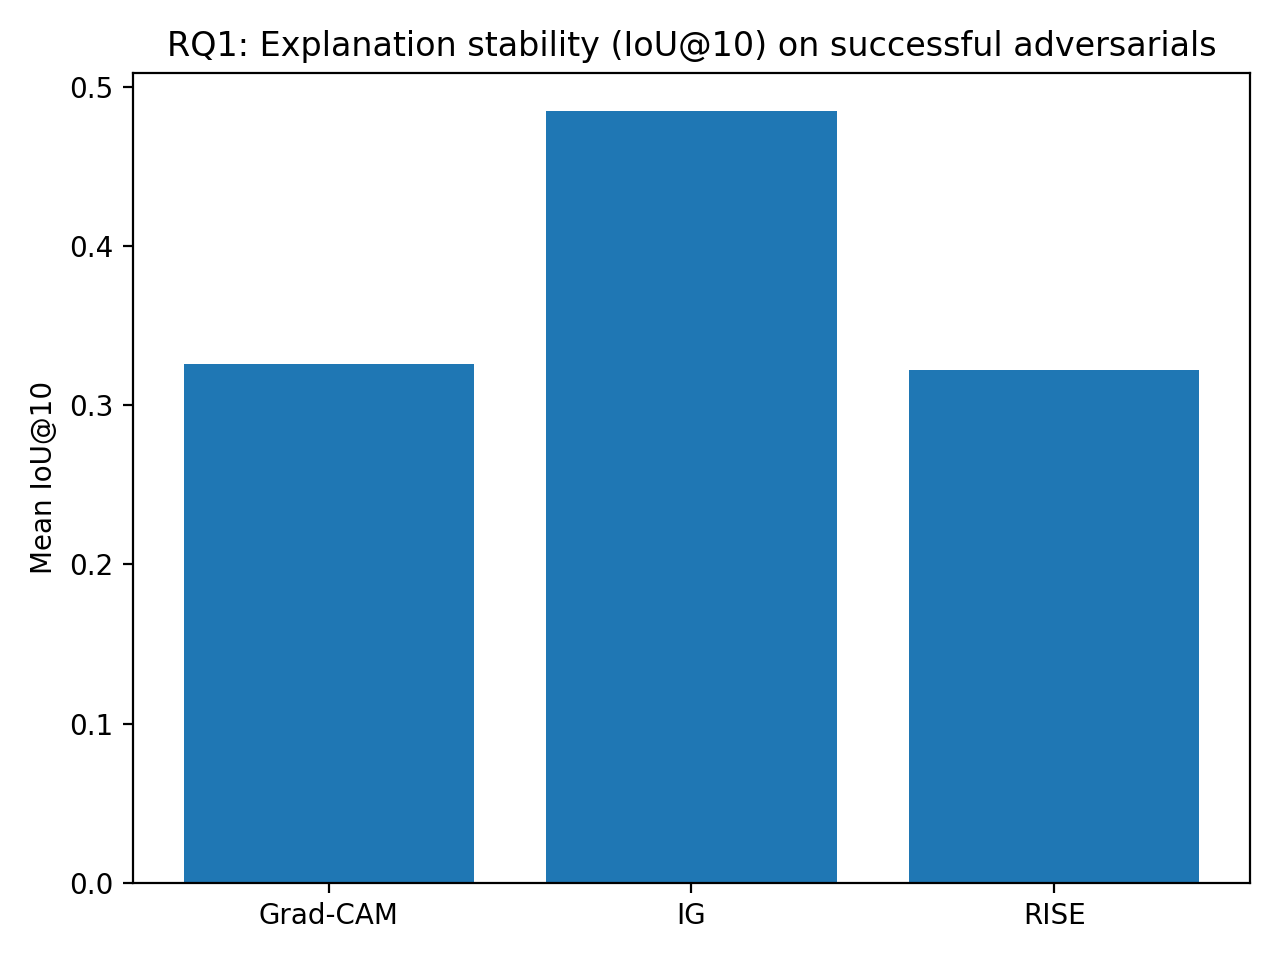
\includegraphics[width=0.85\linewidth]{figures/final_pack/rq1_iou10_adv_mean.png}
  \caption{RQ1: Mean IoU@10 on successful untargeted adversarial examples. Higher values indicate more stable top-ranked salient pixels.}
  \label{fig:rq1_iou10}
\end{figure}

\begin{figure}[t]
  \centering
  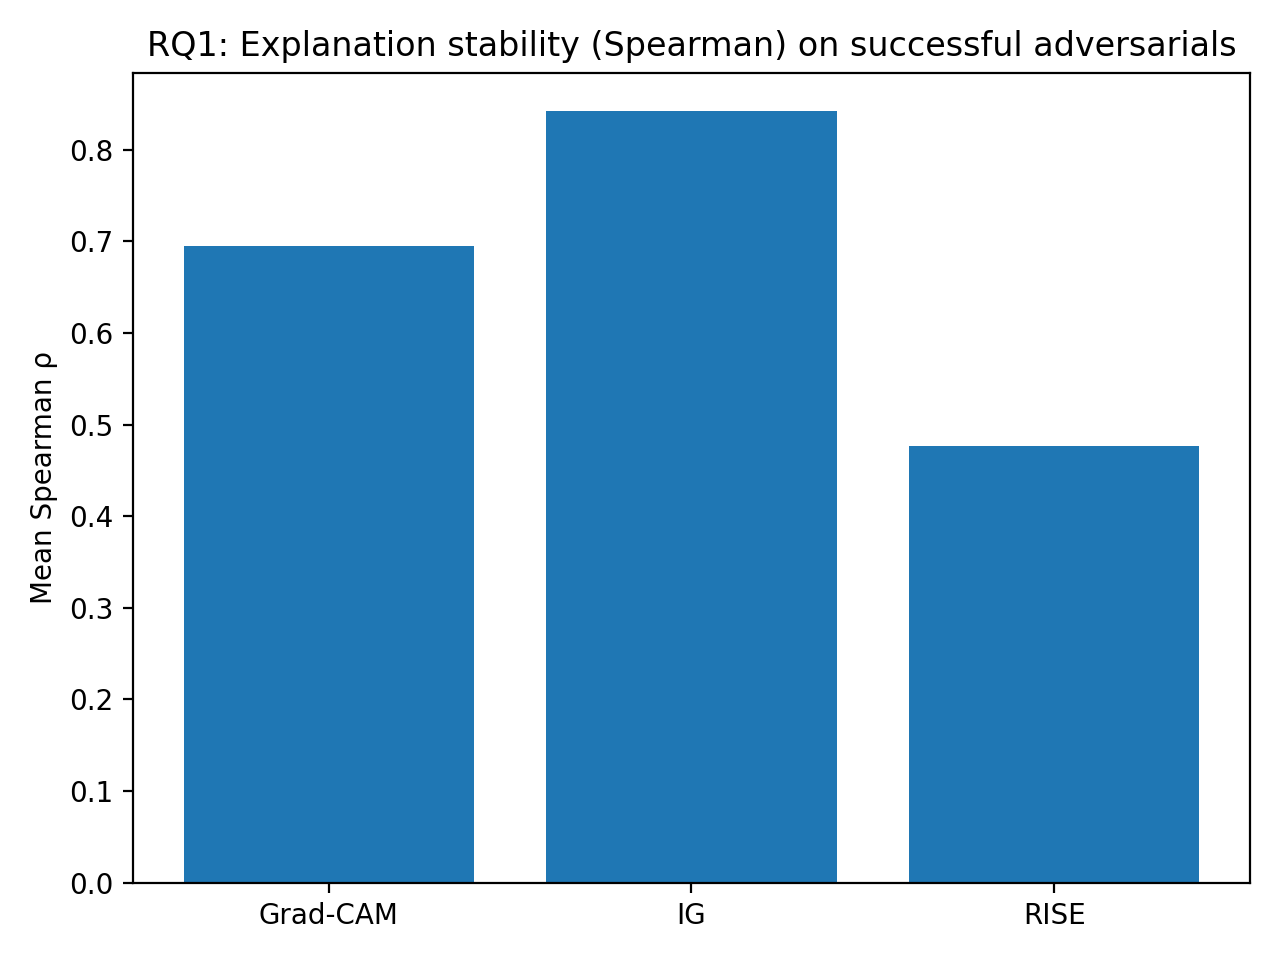
\includegraphics[width=0.85\linewidth]{figures/final_pack/rq1_rho_adv_mean.png}
  \caption{RQ1: Mean Spearman rank correlation on successful untargeted adversarial examples. Higher values indicate more stable attribution ordering.}
  \label{fig:rq1_rho}
\end{figure}

The median values broadly support the same ordering as the means.
This is useful because it suggests that the conclusion is not an artefact of a small number of extreme cases.
Under the present evaluation protocol, IG is consistently the most stable of the three explanation methods, while RISE is the least stable in rank-correlation terms.

\paragraph{Faithfulness under attack.}
Deletion-based faithfulness also deteriorates under successful untargeted attack for all three methods.
For Grad-CAM, deletion AUC falls from clean mean 0.305 to adversarial mean 0.132, giving mean $\Delta$ deletion AUC of \(-0.173\), with median $\Delta$ equal to \(-0.201\).
For IG, deletion AUC falls from clean mean 0.250 to adversarial mean 0.190, giving mean $\Delta$ of \(-0.060\), with median $\Delta$ of \(-0.072\).
For RISE, deletion AUC falls from clean mean 0.257 to adversarial mean 0.093, giving mean $\Delta$ of \(-0.165\), with median $\Delta$ of \(-0.168\).

\begin{figure}[t]
  \centering
  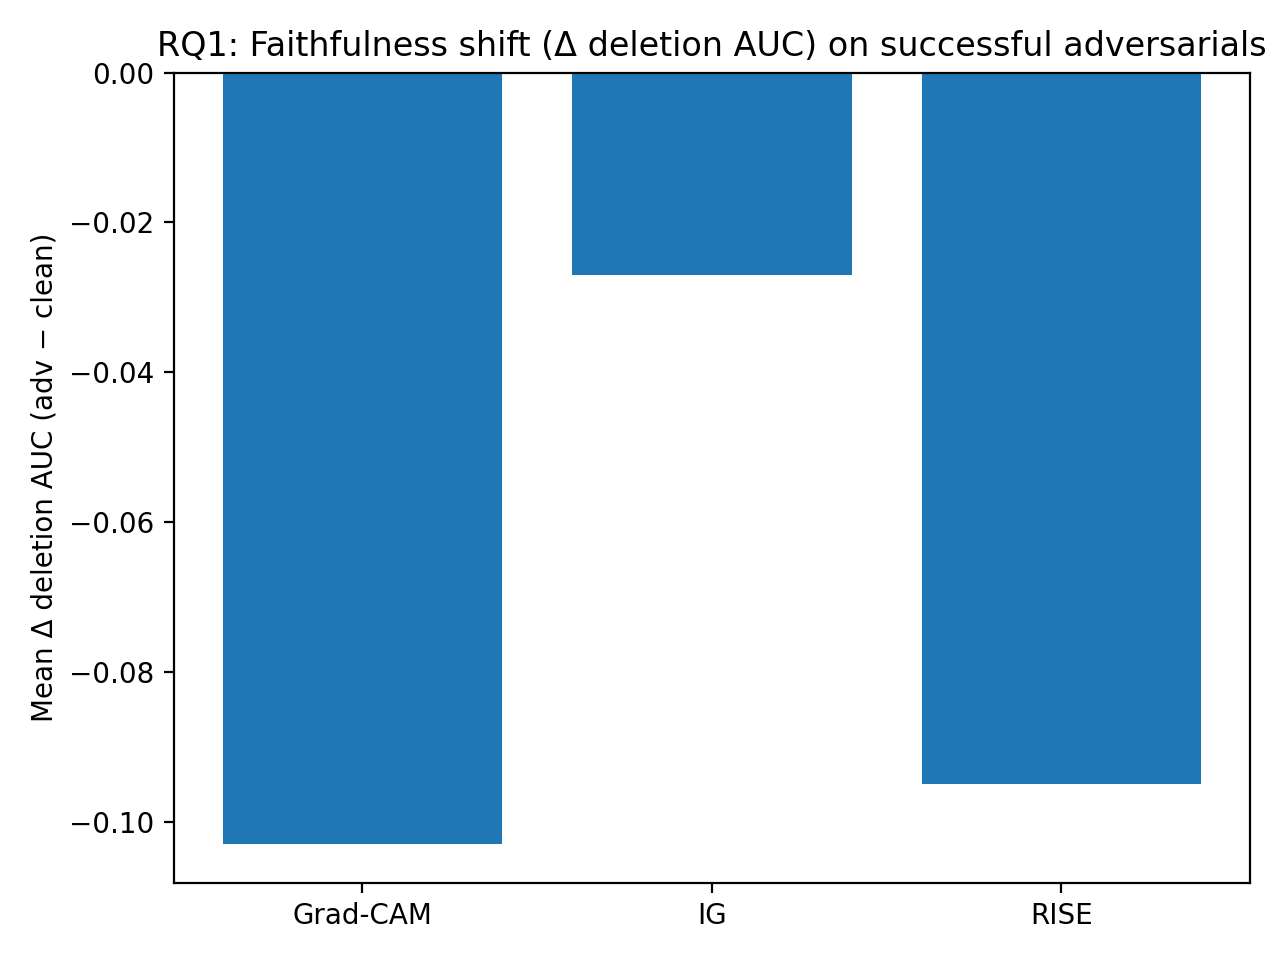
\includegraphics[width=0.85\linewidth]{figures/final_pack/rq1_del_auc_delta_mean.png}
  \caption{RQ1: Mean change in deletion AUC (adversarial minus clean) on successful untargeted adversarial examples. More negative values indicate larger decreases in measured faithfulness under attack.}
  \label{fig:rq1_delauc_delta}
\end{figure}

\paragraph{RQ1 summary.}
The untargeted one-pixel baseline therefore produces successful adversarial examples for which explanation behaviour changes measurably.
The main result is not only that explanation maps shift, but that the magnitude and form of the shift is method-dependent.
IG remains comparatively stable, while all three methods show reduced deletion-based faithfulness on average.

\subsection{RQ2: Can responsibility-map guidance improve one-pixel attacks?}

\subsubsection{Attack effectiveness and query cost}
\begin{table}[t]
\centering
\small
\caption{RQ2 attack outcomes on the eligible CIFAR-10 subset (9{,}213 images): image-wise success rate (ASR) and query cost.}
\label{tab:rq2_attack_summary}
\begin{tabular}{lrrrrr}
\toprule
Run & Eligible & Success & ASR & Median queries (succ) & Median queries (all) \\
\midrule
untargeted & 9,213 & 3,477 & 0.377 & 6,000 & 40,400 \\
fastprior & 9,213 & 1,310 & 0.142 & 70,848 & 70,848 \\
rise-guided & 9,213 & 3,477 & 0.377 & 6,400 & 40,400 \\
\bottomrule
\end{tabular}

\end{table}


\begin{figure}[t]
  \centering
  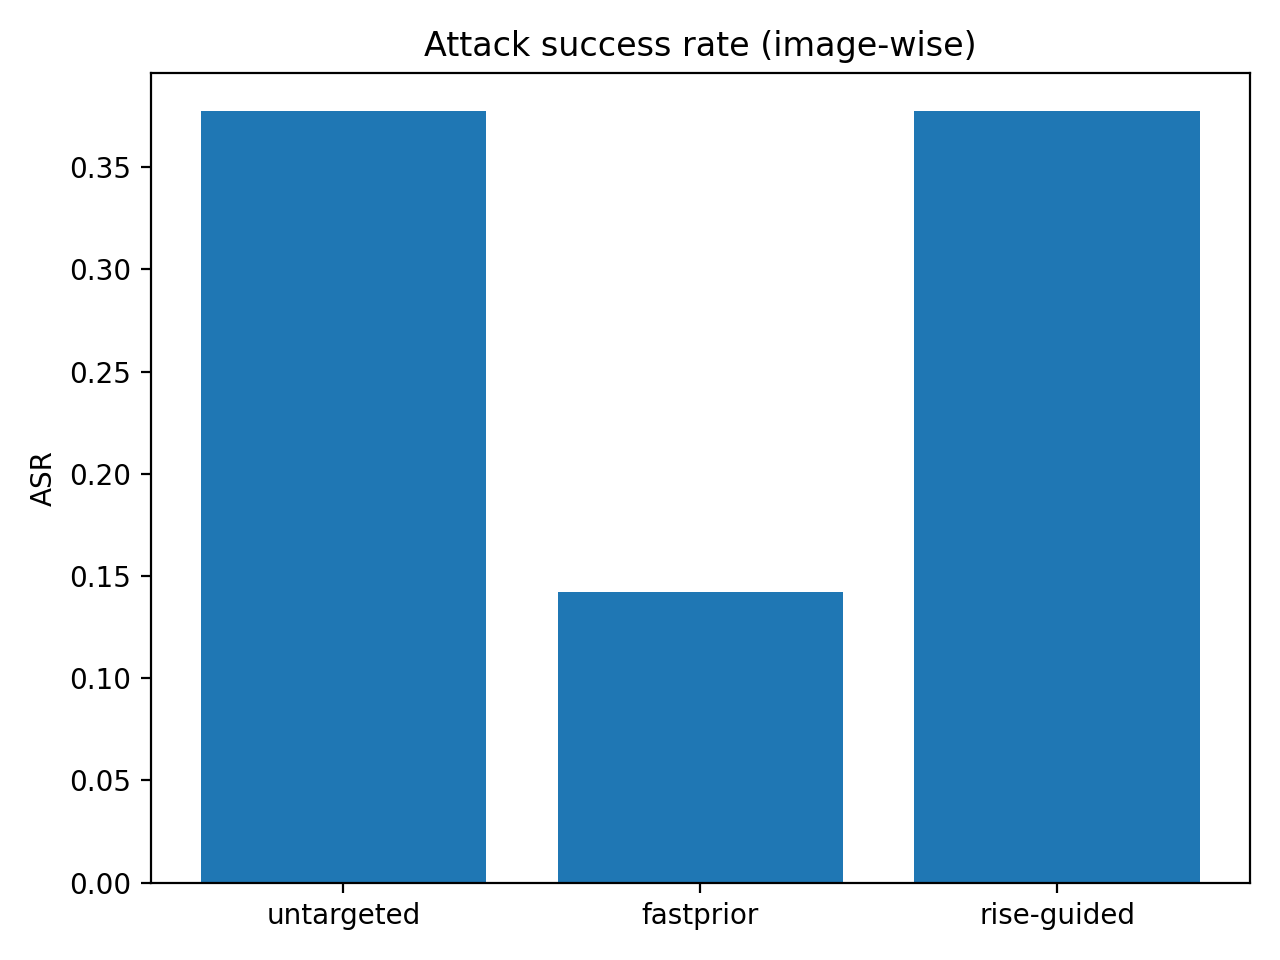
\includegraphics[width=0.85\linewidth]{figures/final_pack/asr_by_run.png}
  \caption{Attack success rate across the three main 10k-scale runs.}
  \label{fig:rq2_asr_by_run}
\end{figure}

\begin{figure}[t]
  \centering
  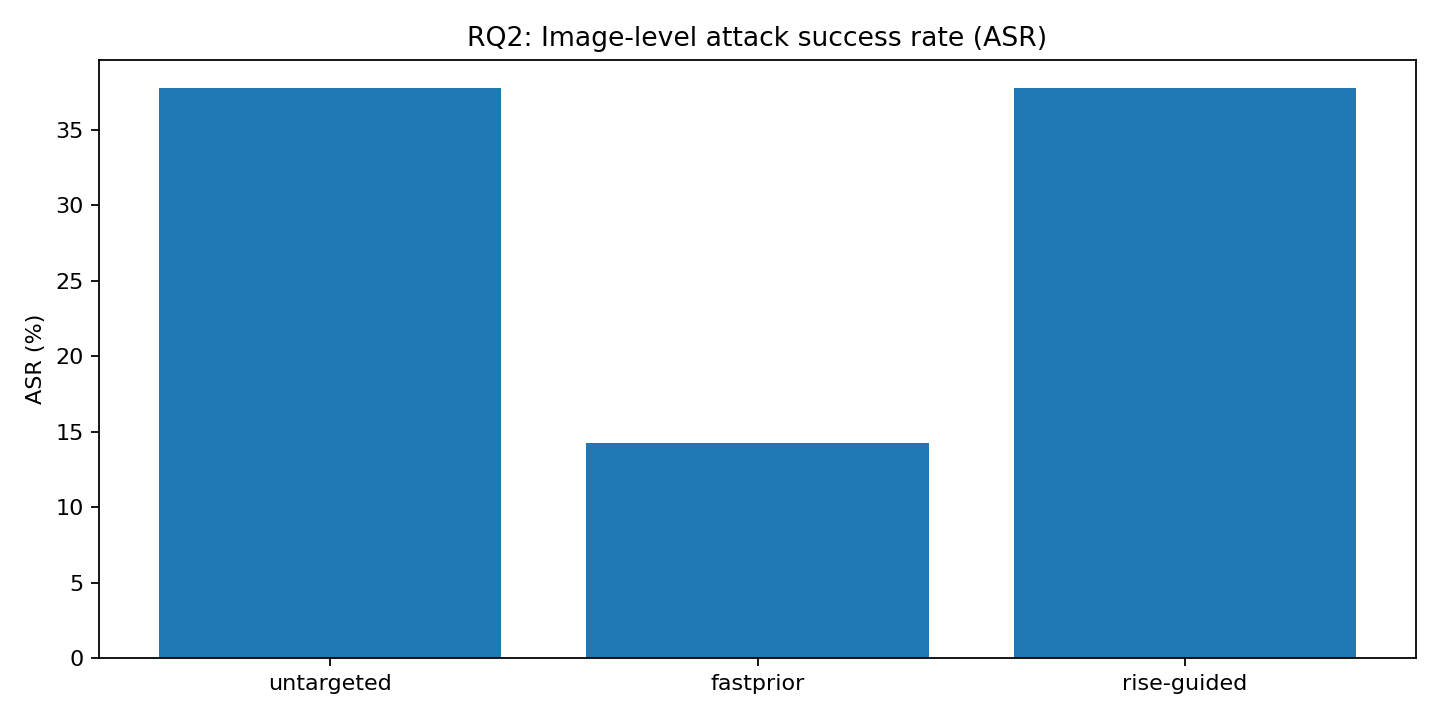
\includegraphics[width=0.85\linewidth]{figures/final_pack/rq2_asr_image_percent.png}
  \caption{Image-wise attack success rate (ASR) on the 9{,}213 eligible CIFAR-10 test images.}
  \label{fig:rq2_asr}
\end{figure}

\begin{figure}[t]
  \centering
  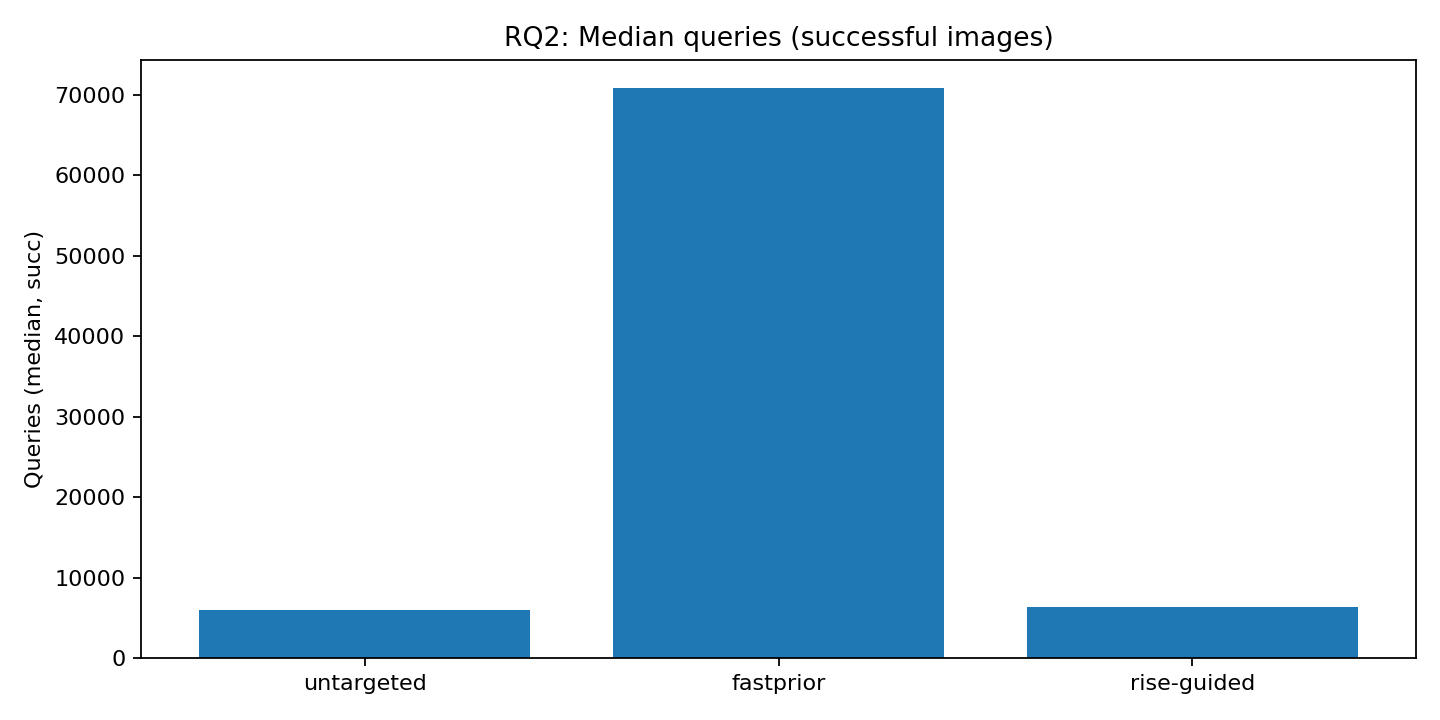
\includegraphics[width=0.85\linewidth]{figures/final_pack/rq2_queries_median_success.png}
  \caption{Median query cost among successful attacks. Lower values indicate more efficient successful attacks.}
  \label{fig:rq2_queries_succ}
\end{figure}

Table~\ref{tab:rq2_attack_summary} and \Cref{fig:rq2_asr_by_run,fig:rq2_asr,fig:rq2_queries_succ} summarise the main success--cost comparison.
The untargeted DE baseline achieves image-wise ASR 0.3774, corresponding to 3{,}477 successful attacks out of 9{,}213 eligible images.
Its median query cost is 40{,}400 over all eligible images and 6{,}000 over successful images.
The corresponding median generation count is 100 over all eligible images but only 14 over successful images, indicating that many failures run to the generation limit while successful attacks often stop much earlier.

The fastprior variant reduces image-wise ASR to 0.1422, corresponding to 1{,}310 successful images.
Its median query cost is 70{,}848 both overall and among successful cases, reflecting the fixed-budget design.
The median generation count is likewise 40 both overall and among successful cases.
At the target level, fastprior records 1{,}482 successful targets out of 82{,}917 target attempts, corresponding to target-wise success rate 0.0179.
This confirms that the method does find successful target flips, but that these do not translate efficiently into broad image-wise success.

The RISE-guided DE variant matches the untargeted baseline in image-wise ASR at 0.3774, again corresponding to 3{,}477 successful images.
Its overall median query cost remains 40{,}400, while the median cost among successful cases rises slightly to 6{,}400.
The median generation count is 100 over all eligible images and 15 among successful cases.
This means that, at the level of these aggregate medians, RISE-guided search preserves the baseline success rate but does not improve the overall success--cost frontier.

\subsubsection{Explanation behaviour on successful adversarial examples}
\begin{table}
\begingroup
\hbadness=10000
\hfuzz=100pt
\setlength{\emergencystretch}{2em}
\sloppy
[t]
\centering
\scriptsize
\setlength{\tabcolsep}{3pt}
\renewcommand{\arraystretch}{1.15}
\small
\resizebox{0.92\linewidth}{!}{%
\begin{minipage}{\linewidth}
\caption{RQ2 explanation stability on successful adversarial examples (means). Higher IoU@10 and Spearman indicate more stable explanations.}
\label{tab:rq2_stability_means}
\begin{tabular}{lrrrrrr}
\toprule
Run & IoU@10 GC & IoU@10 IG & IoU@10 RISE & Spearman GC & Spearman IG & Spearman RISE \\
\midrule
untargeted & 0.326 & 0.485 & 0.322 & 0.695 & 0.842 & 0.477 \\
fastprior & 0.517 & 0.532 & 0.367 & 0.839 & 0.866 & 0.525 \\
rise-guided & 0.325 & 0.484 & 0.296 & 0.693 & 0.842 & 0.445 \\
\bottomrule
\end{tabular}

\end{minipage}}
\endgroup
\end{table}

\begin{table}[t]
\centering
\small
\setlength{\tabcolsep}{4pt}
\renewcommand{\arraystretch}{1.15}
\caption{RQ2 faithfulness shift under attack: mean change in deletion AUC (adversarial minus clean) on successful adversarial examples. More negative indicates a larger drop.}
\label{tab:rq2_del_delta}
\begin{tabular}{lrrr}
\toprule
Run & $\Delta$DelAUC GC & $\Delta$DelAUC IG & $\Delta$DelAUC RISE \\
\midrule
untargeted & -0.173 & -0.060 & -0.165 \\
fastprior & -0.148 & -0.069 & -0.148 \\
rise-guided & -0.173 & -0.060 & -0.159 \\
\bottomrule
\end{tabular}
\end{table}


\begin{figure}[t]
  \centering
  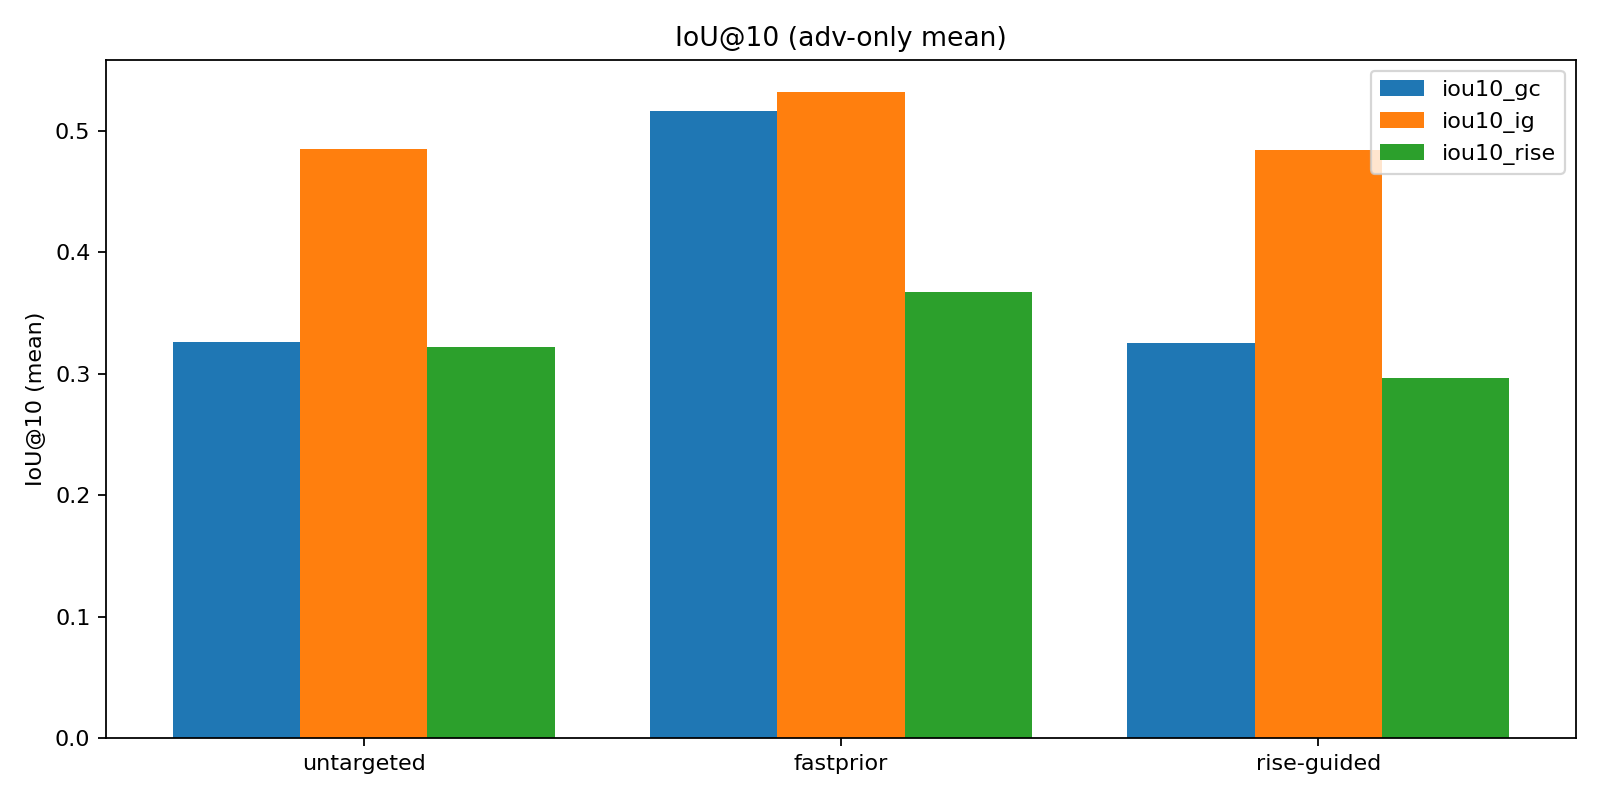
\includegraphics[width=0.85\linewidth]{figures/final_pack/rq2_iou10_adv_mean.png}
  \caption{Mean IoU@10 of explanation maps on successful adversarial examples across attack variants.}
  \label{fig:rq2_iou10}
\end{figure}

\begin{figure}[t]
  \centering
  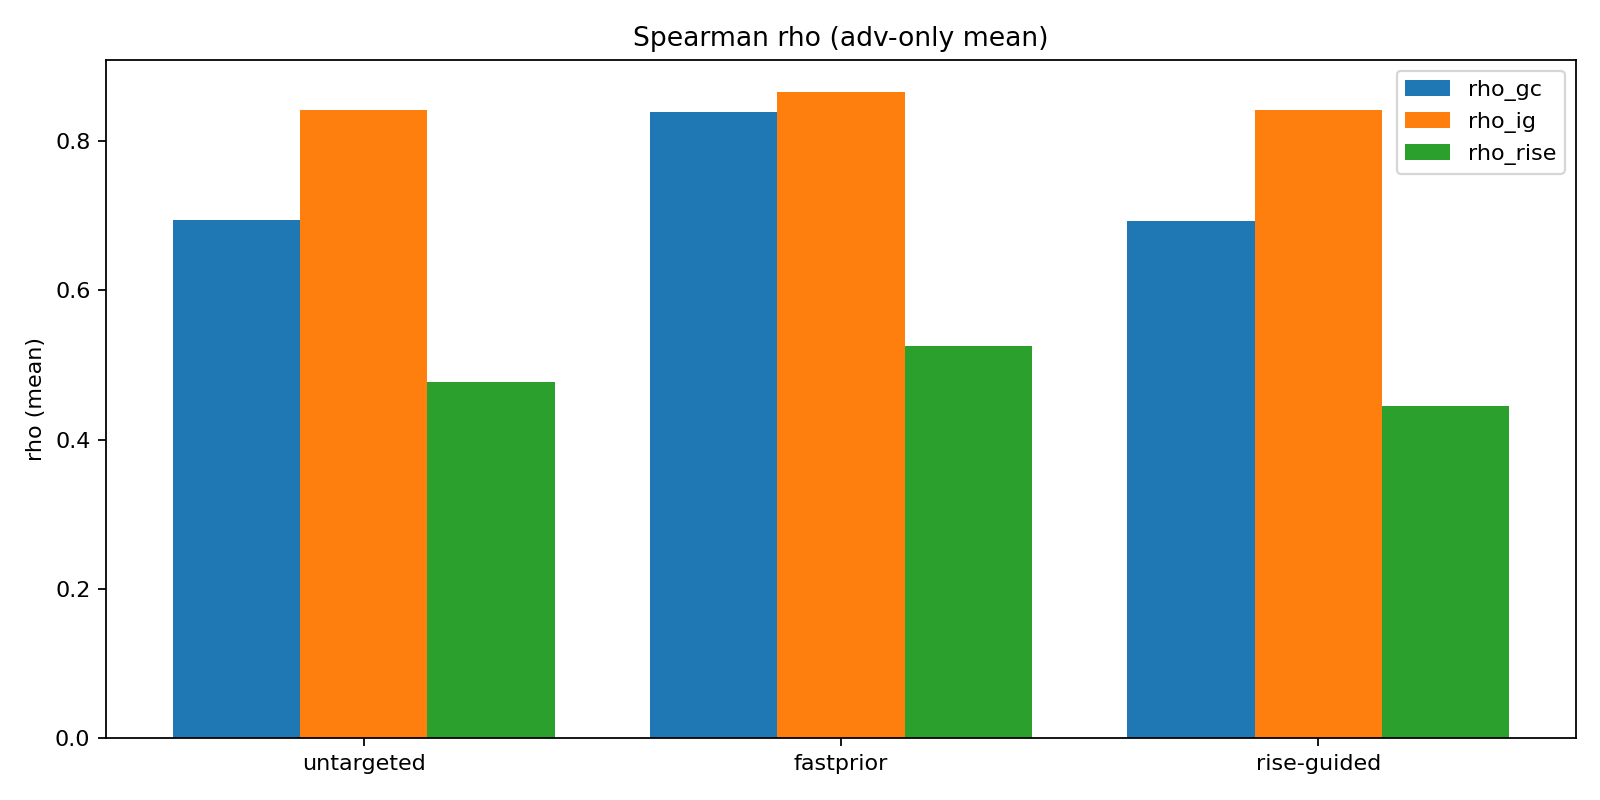
\includegraphics[width=0.85\linewidth]{figures/final_pack/rq2_rho_adv_mean.png}
  \caption{Mean Spearman rank correlation on successful adversarial examples across attack variants.}
  \label{fig:rq2_rho}
\end{figure}

\begin{figure}[t]
  \centering
  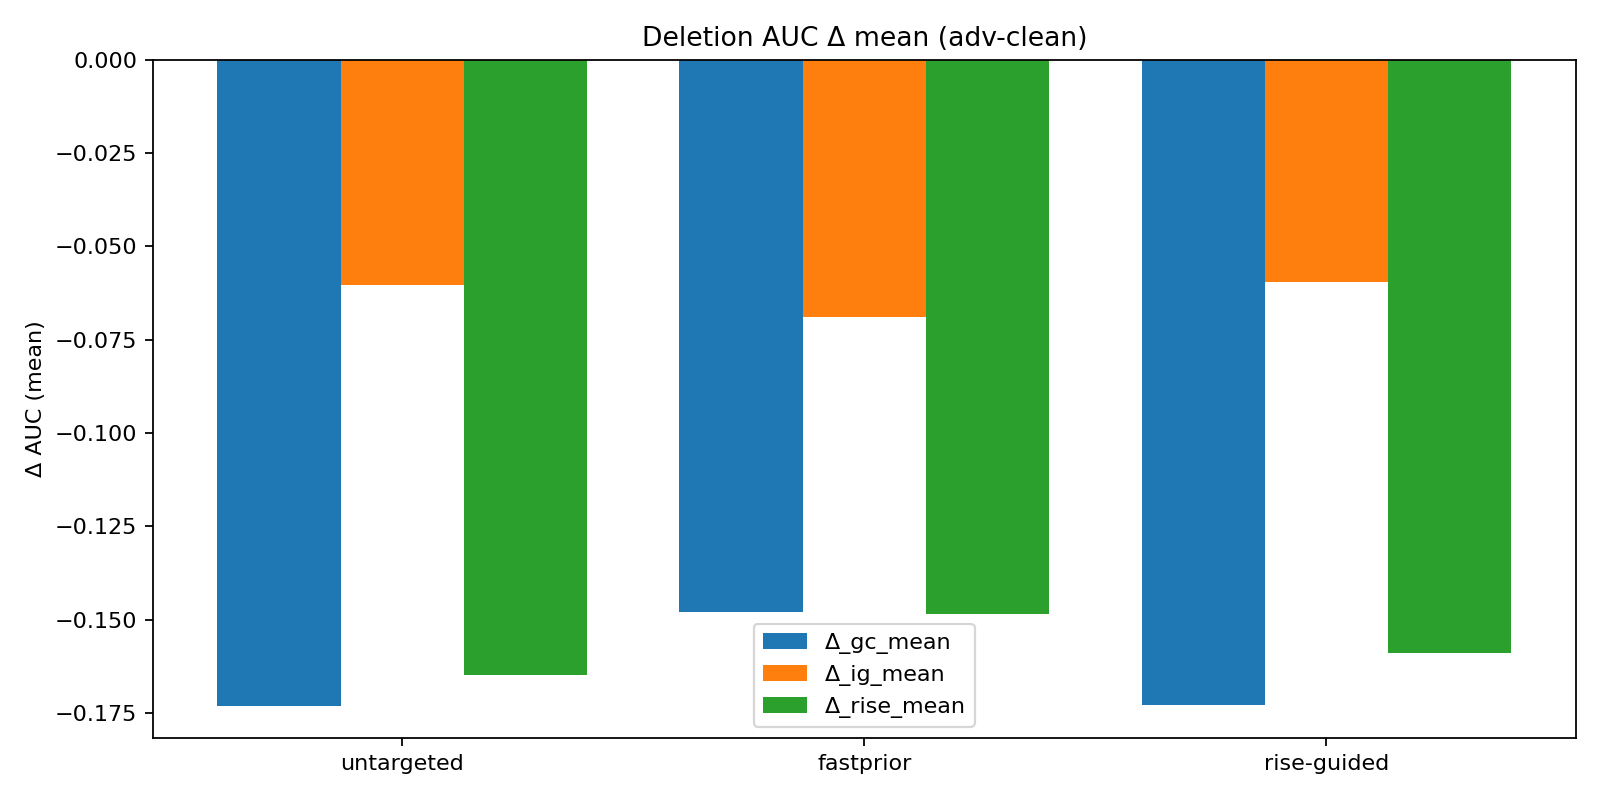
\includegraphics[width=0.85\linewidth]{figures/final_pack/rq2_del_auc_delta_mean.png}
  \caption{Mean change in deletion AUC (adversarial minus clean) across attack variants and explanation methods.}
  \label{fig:rq2_delauc_delta}
\end{figure}

Table~\ref{tab:rq2_stability_means}, Table~\ref{tab:rq2_del_delta}, and \Cref{fig:rq2_iou10,fig:rq2_rho,fig:rq2_delauc_delta} compare explanation behaviour across successful adversarial subsets from the three attack configurations.

Integrated Gradients remains the most stable method in rank-correlation terms across all runs: mean Spearman $\rho$ is 0.842 for untargeted, 0.866 for fastprior, and 0.842 for RISE-guided, with corresponding medians 0.849, 0.873, and 0.849.
Fastprior shows the highest stability values across all three explanation methods when measured on its successful subset.
For example, its IoU@10 values are 0.517, 0.532, and 0.367 for Grad-CAM, IG, and RISE respectively, compared with 0.326, 0.485, and 0.322 for the untargeted baseline.
Its median Spearman values are also notably high, especially for Grad-CAM and IG at 0.921 and 0.873 respectively.

The RISE-guided variant remains very close to the untargeted baseline for Grad-CAM and Integrated Gradients.
For RISE itself, however, stability decreases under guidance: mean IoU@10 drops from 0.322 to 0.296 and median IoU@10 drops from 0.308 to 0.283, while mean Spearman $\rho$ drops from 0.477 to 0.445 and median Spearman $\rho$ drops from 0.503 to 0.467.

Deletion-based faithfulness degrades under successful attack for all runs and methods.
For the untargeted run, mean $\Delta$ deletion AUC is \(-0.173\), \(-0.060\), and \(-0.165\) for Grad-CAM, IG, and RISE respectively.
For fastprior, the corresponding means are \(-0.148\), \(-0.069\), and \(-0.148\).
For RISE-guided DE, they are \(-0.173\), \(-0.060\), and \(-0.159\).
The medians show the same overall direction of change, although the exact magnitudes differ somewhat across methods and runs.

\subsection{Results summary}
The results provide four direct empirical findings.
First, successful untargeted one-pixel attacks are associated with measurable explanation change, with IG more stable than Grad-CAM and RISE under the present metrics.
Second, the frozen artefacts show exact matching between successful attack counts and adversarial explanation rows, which strengthens confidence in the consistency of the reporting pipeline.
Third, fastprior improves explanation stability on its successful subset but does so together with lower image-wise success, fixed high cost, and weak target-wise conversion.
Fourth, RISE-guided DE preserves headline success rate relative to the untargeted baseline but does not improve the overall success--cost frontier and reduces RISE-based stability on its successful subset.
These results are interpreted in depth in the next chapter.
